\documentclass[10pt,a4paper,twocolumn]{article}

% Page layout — tight margins for two-column
\usepackage[margin=1.8cm,columnsep=0.6cm]{geometry}

% Modern font: Palatino text + matching math
\usepackage[utf8]{inputenc}
% \usepackage[T1]{fontenc}
% \usepackage{newpxtext}    % Palatino text
\usepackage{newpxmath}    % Palatino math

% Packages
\usepackage{amsmath}
\let\Bbbk\relax        % Resolve newpxmath/amssymb conflict
\usepackage{amssymb}
\usepackage{graphicx}
\usepackage{booktabs}
\usepackage{hyperref}
\usepackage{float}
\usepackage{algorithm}
\usepackage{algpseudocode}
\usepackage{listings}
\usepackage{xcolor}
\usepackage{caption}
\usepackage{multirow}
\usepackage{enumitem}
\usepackage{microtype}    % Better typography
\usepackage{flushend}     % Balance last page columns

% Hyphenation and line breaking
\tolerance=1500
\emergencystretch=1.5em
\hyphenpenalty=50

% Caption styling
\captionsetup{
    font=small,
    labelfont=bf,
    labelsep=period,
    justification=raggedright,
    singlelinecheck=false
}

% Code listing style
\lstset{
    basicstyle=\ttfamily\scriptsize,
    keywordstyle=\color{blue!80!black},
    commentstyle=\color{gray!70!black},
    breaklines=true,
    frame=single,
    xleftmargin=0.5em,
    xrightmargin=0.5em,
    numbers=none,
    aboveskip=0.5em,
    belowskip=0.5em
}

% Hyperref styling
\hypersetup{
    colorlinks=true,
    linkcolor=blue!60!black,
    citecolor=green!40!black,
    urlcolor=blue!60!black
}

% Abstract styling: one step smaller, centered
\renewenvironment{abstract}
  {\centerline{\large\bfseries\abstractname}\vspace{0.5em}\small\begin{center}\begin{minipage}{0.92\textwidth}}
  {\end{minipage}\end{center}\par}

% Compact sections
\usepackage{titlesec}
\titlespacing*{\section}{0pt}{1.2ex plus 0.3ex minus 0.2ex}{0.6ex plus 0.1ex}
\titlespacing*{\subsection}{0pt}{0.8ex plus 0.2ex minus 0.1ex}{0.4ex plus 0.1ex}
\titleformat{\section}{\normalfont\large\bfseries}{\thesection}{0.5em}{}
\titleformat{\subsection}{\normalfont\normalsize\bfseries}{\thesubsection}{0.5em}{}
\titlespacing*{\paragraph}{0pt}{0.6ex plus 0.2ex minus 0.1ex}{0.5em}

\title{\textbf{Higher-Order Protein Feature Co-occurrence at AlphaFold Scale}}

\author{E.\ Ahmic}

\date{September 2026 (version 2)}

\begin{document}

\twocolumn[
\maketitle
\vspace{-1em}
\begin{abstract}
The AlphaFold database contains over 200 million predicted protein structures, but systematically discovering which protein features co-occur across this universe is computationally prohibitive: a standard boolean representation requires over 200\,GB, exceeding GPU memory capacity. ET-miner compresses the transaction data into a sparse representation and loads bitvectors onto the GPU, where they remain resident across all $K$-levels; only lightweight metadata (prefix groups and result indices) crosses the PCIe bus at each iteration. With a base vocabulary of 1,002 features, this enables exhaustive Apriori computation across 76.9 million proteins in 43.9\,minutes (excluding feature extraction) on a single NVIDIA GeForce RTX 3090, revealing 26.8 million co-occurrence patterns reaching $K{=}22$. A permutation null model at 0.001\% support (100 permutations preserving per-protein feature counts) never produces an itemset beyond $K{=}6$, whereas the biological data contain 88,745 itemsets with $K{\geq}7$ (empirical $p{\approx}0.01$; see Section~\ref{sec:null-model} for scope). All results reported here come from a single complete execution of the pipeline on freshly downloaded data (September 2026), whose artifacts are deposited with the code.
\end{abstract}
\vspace{1em}
]

%==============================================================================
\section{Introduction}
\label{sec:introduction}
%==============================================================================

The completion of the AlphaFold Protein Structure Database~\cite{jumper2021,varadi2022} represents one of the largest expansions of biological knowledge in history. With predicted structures for over 200 million proteins spanning virtually all known organisms, the database transforms structural biology from a field constrained by experimental bottleneck to one overwhelmed by data abundance. Yet while structure \emph{prediction} has been solved at scale, structure \emph{mining}---the systematic discovery of which structural and functional features co-occur across the protein universe---remains largely unexplored. Protein domain co-occurrence has been studied primarily through pairwise network approaches~\cite{wang2011,coin2009} and small-scale spatial pattern mining~\cite{meysman2015}, but no existing work performs exhaustive higher-order co-occurrence analysis at proteome scale.

The question we address is deceptively simple: \textbf{which combinations of protein features appear together more often than expected across hundreds of millions of proteins?} A protein annotated with a DEAD-box helicase domain (PF00270), RNA helicase activity (GO:0003724), and innate immune response (GO:0045087) represents a specific functional configuration. This 3-feature combination appears in 1,234 of the proteins mined here; when such a combination recurs across distant evolutionary lineages, it reveals a conserved molecular machine, one that natural selection has independently assembled or maintained. Discovering such patterns at the scale of the entire protein universe requires a computational approach fundamentally different from existing tools.

Frequent itemset mining (FIM) is the natural framework for this problem. Each protein becomes a \emph{transaction}, its annotated features (Pfam domains, Gene Ontology terms, structural properties) become \emph{items}, and the Apriori algorithm~\cite{agrawal1994} systematically discovers all feature combinations appearing in at least a minimum number of proteins. GPU-accelerated FIM systems~\cite{luna2019,zhang2011,chon2018,djenouri2019,acmsurvey2021} have achieved $50$--$350\times$ speedups over classical CPU algorithms such as Eclat~\cite{zaki2000,zaki1997} and FP-Growth~\cite{han2000}, but all existing GPU implementations were evaluated on datasets of at most a few million real transactions, one to two orders of magnitude smaller than our proteome dataset. The standard dense boolean matrix representation requires ${\sim}206$\,GB for 205.6~million proteins with 1,002 features (one byte per boolean entry), far exceeding the 24\,GB of the GPU used here.

Figure~\ref{fig:concept} illustrates this formulation: each protein is a transaction of annotated features, forming a sparse boolean matrix---a representation central to a broad family of pattern-discovery and Boolean matrix methods~\cite{miettinen2020}---on which support counting reduces to bitwise AND and population count.

\begin{figure*}[t]
    \centering
    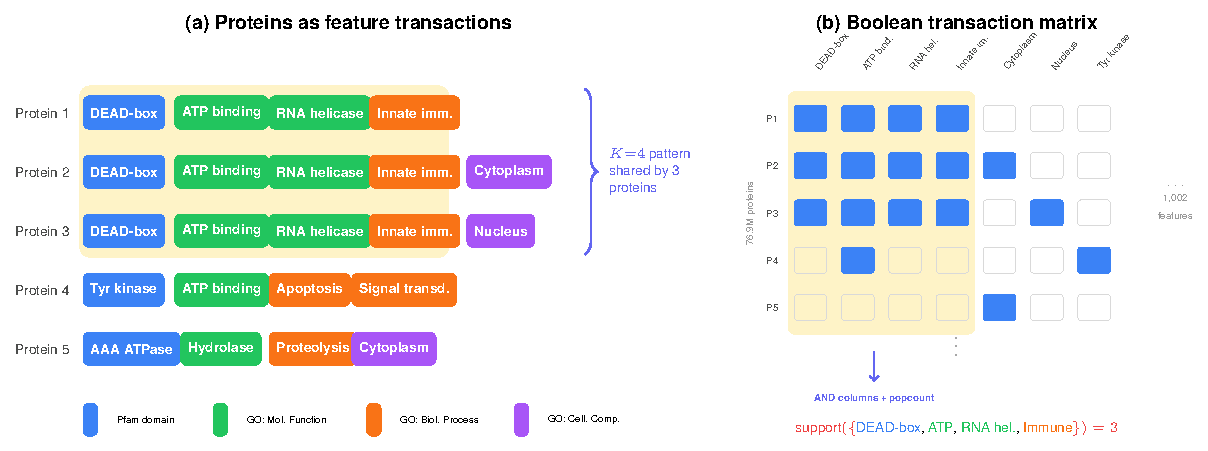
\includegraphics[width=\textwidth]{figures/concept_figure.pdf}
    \caption{Frequent itemset mining applied to protein annotations.
    \textbf{(a)}~Each protein is treated as a transaction whose items are its annotated Pfam domains, GO terms, and structural properties.
    A $K{=}4$ pattern (yellow highlight) is shared by three proteins.
    \textbf{(b)}~The transaction database as a boolean matrix (76.9M proteins $\times$ 1,002 features).
    Support counting for any candidate itemset reduces to a column-wise AND followed by a population count.}
    \label{fig:concept}
\end{figure*}

ET-miner solves this through three innovations: (1)~a compressed sparse row (CSR) representation constructed directly from the transaction list, reducing 206\,GB to ${\sim}5.1$\,GB in coordinate form; (2)~on-GPU conversion to bitvectors where support counting reduces to bitwise AND and population count, operations GPUs execute natively; and (3)~a GPU-accelerated mining loop where bitvectors remain GPU-resident across $K$-levels, with only lightweight metadata (prefix groups and result indices) crossing the PCIe bus, greatly reducing the transfer overhead that dominates prior GPU FIM systems. Applied to 76.9~million multi-feature proteins, ET-miner discovers the complete feature co-occurrence landscape in 43.9\,minutes of mining on a single NVIDIA GeForce RTX 3090, enabling systematic exploration of higher-order protein functional modularity across the protein universe.

%==============================================================================
\section{Methods}
\label{sec:methods}
%==============================================================================

\subsection{Dataset and Feature Vocabulary}

The AlphaFold Protein Structure Database~\cite{varadi2024} provides predicted structures for 214 million proteins across UniProt. We processed the 205,620,298 AlphaFold DB entries (of 214,683,829) whose mean predicted local distance difference test (pLDDT) confidence is at least 50 and obtained their annotations (Pfam domain assignments and Gene Ontology (GO) terms) from the UniProt~\cite{uniprot2023} cross-reference pipeline (TrEMBL release 2026\_01, 202,556,314 entries, retrieved from the UniProt archive on 2 September 2026). Protein annotations comprise Pfam~\cite{mistry2021} domain assignments, Gene Ontology~\cite{go2023} terms, and pLDDT confidence scores. The feature vocabulary comprises the 500 most frequent Pfam domains and the 500 most frequent GO terms (drawn from 24{,}291 Pfam and 25{,}993 GO families observed across the corpus), together with 6 pLDDT confidence bins (three on the mean pLDDT and three on the fraction of high-confidence residues; the low mean-pLDDT bin is removed by the pLDDT${\geq}50$ filter and the three fraction bins are not assigned by the metadata-based extraction, which sees only the per-protein mean, so only the mean-pLDDT bins 50--90 and ${>}90$ are populated), for 1{,}006 defined items; the minimum support threshold of 8 proteins is applied during \emph{mining}, not during vocabulary construction. Feature extraction streamed the 149.8\,GiB compressed flat file and reduced it to the record lines it parses (48\,minutes, network-bound), restricted it in two filtering passes (29\,minutes) to the 90.5 million pLDDT-passing proteins with Pfam or GO cross-references, and built the transactions in 9.3\,minutes of extractor time (10.4\,minutes wall-clock; 162,865 proteins/s); this preprocessing is separate from the 43.9\,minute mining runtime reported below. Exact itemset counts and $K$-distributions may vary with different UniProt releases due to ongoing annotation updates.

Each protein is represented as a transaction: a set of integer item identifiers corresponding to its annotated features. The feature vocabulary is shown in Table~\ref{tab:features}.

\begin{table}[h]
\caption{Feature vocabulary composition: 1,006 items are defined (6 pLDDT confidence bins, 500 Pfam domains, 500 GO terms) and 1,002 pass the support threshold of 8 proteins (all 1,000 Pfam/GO items plus 2 pLDDT bins; the other 4 pLDDT bins are empty).}
\label{tab:features}
\centering
\resizebox{\columnwidth}{!}{%
\begin{tabular}{@{}llrr@{}}
\toprule
Feature Type & Source & Defined & Frequent \\
\midrule
Pfam domains & InterPro/Pfam & 500 & 500 \\
GO terms & Gene Ontology & 500 & 500 \\
pLDDT confidence bins & AlphaFold & 6 & 2 \\
\midrule
\textbf{Total} & & \textbf{1,006} & \textbf{1,002} \\
\bottomrule
\end{tabular}%
}
\end{table}

Of the 205,620,298 total proteins, 76,890,945 (37.4\%) have more than one annotated feature under this vocabulary and form the transaction set mined in this work.

\subsection{Architecture Overview}

ET-miner implements a GPU-accelerated Apriori algorithm with a CPU path (boolean matrices with vectorized column operations, or a sparse variant) and a GPU path that builds bitvectors on-GPU directly from CSR and keeps them GPU-resident across all $K$-levels, with only lightweight metadata crossing the PCIe bus; the GPU path has single-GPU, multi-GPU (candidate-split or row-split) and sparse-CSR variants. The GPU path is the primary contribution and was used for all results reported in this paper: the single-GPU variant for the mining campaign, and the row-split variant (transactions partitioned across two GPUs, partial counts summed per candidate) for the permutation null model and the per-level itemset exports. We chose Apriori's level-wise structure over FP-Growth~\cite{han2000} specifically because its support counting step maps naturally to GPU SIMD parallelism, while FP-tree construction is inherently sequential. Figure~\ref{fig:architecture} illustrates the end-to-end pipeline.

\begin{figure*}[t]
    \centering
    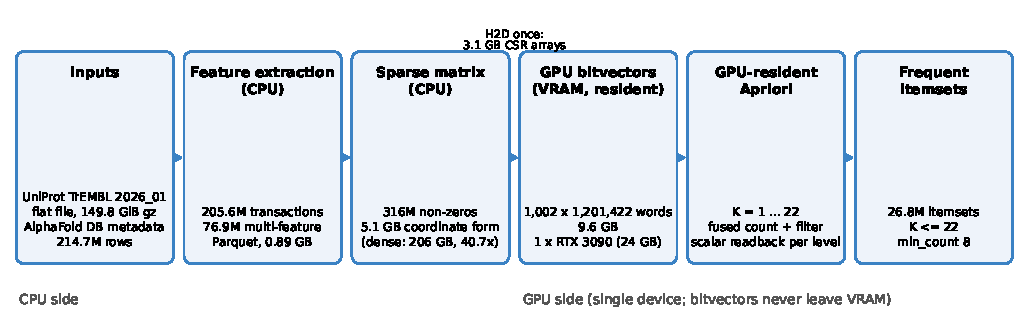
\includegraphics[width=\textwidth]{figures/architecture.pdf}
    \caption{ET-miner pipeline: Parquet transactions are compressed to sparse format and converted to GPU-resident bitvectors. Support counting executes on-GPU; prefix group construction and result collection cross the PCIe bus at each $K$-level.}
    \label{fig:architecture}
\end{figure*}

\subsection{Sparse Matrix Construction}

Rather than constructing the full dense matrix, we build a compressed sparse row (CSR) representation that stores only non-zero entries, recording which features each protein actually has. The construction streams through the Parquet file, identifies frequent features, determines which proteins carry each feature, and encodes these relationships as coordinate pairs converted to CSR format. For the 76.9M-protein mining subset, the resulting matrix contains 316~million non-zero entries occupying ${\sim}5.1$\,GB in coordinate format (two 64-bit integers per entry), a ${\sim}15\times$ reduction from the ${\sim}77$\,GB dense representation of that same subset (one byte per boolean entry); relative to the ${\sim}206$\,GB dense matrix of the full 205.6M-protein set it is ${\sim}40\times$ smaller. The bit-packed dense form is smaller (${\sim}26$\,GB for the full set, 9.6\,GB for the mining subset) but still exceeds the CSR footprint.

\subsection{GPU-Resident Bitvector Representation}
\label{sec:bitvec}

For each protein feature, we store a compact binary list indicating which proteins possess that feature. Testing whether two features co-occur then reduces to a fast bitwise AND operation. With 205.6M proteins and 1,002 features, the full bitvector matrix would occupy ${\sim}26$\,GB of GPU memory; the 76.9M-protein mining subset used in every run occupies 9.6\,GB, built directly on-GPU from the CSR arrays after a one-time host-to-device copy (${\sim}3.1$\,GB of 64-bit row pointers and column indices).

Support counting for any candidate itemset $\{A, B, C\}$ then reduces to:
\begin{align*}
    \text{support}(\{A, B, C\}) = \;&\text{popcount}(\text{bitvec}[A] \\
    &\;\texttt{AND}\; \text{bitvec}[B] \\
    &\;\texttt{AND}\; \text{bitvec}[C])
\end{align*}
where \texttt{popcount} counts how many proteins share all features in the candidate set, replacing the need to iterate over every protein individually.

\subsection{GPU-Accelerated Mining}

Traditional approaches generate candidates on the CPU, transfer them to the GPU for counting, return results, and filter on the CPU, repeating this cycle at every level. ET-miner keeps bitvectors GPU-resident across all $K$-levels, performing support counting and filtering on-GPU while prefix group construction and result collection occur on the CPU with lightweight PCIe transfers. At each $K$-level:

\begin{itemize}[leftmargin=*]
    \item $K{=}1$: Count proteins for each feature; retain those above the
          support threshold.
    \item $K{=}2$: Test all feature pairs; retain frequent pairs.
    \item $K{\geq}3$: Group candidates by shared prefix, test each group,
          retain those meeting the threshold.
\end{itemize}

Because bitvectors remain GPU-resident, the per-level PCIe traffic is limited to prefix group metadata and result indices---orders of magnitude less than conventional approaches that transfer full candidate sets and support arrays each iteration~\cite{zhang2011,chon2018,djenouri2019}. Per-level transfer details
are provided in Appendix~\ref{app:gpu-details}.

\noindent In summary, the algorithm loads bitvectors onto the GPU once, where they remain resident across all $K$-levels. Each iteration transfers only lightweight prefix group metadata and result indices across the PCIe bus, while the bulk computation stays on-GPU. Full pseudocode is provided in Appendix~\ref{app:pseudocode}. For multi-GPU configurations, ET-miner can replicate bitvectors on each device and distribute candidates by index range, or partition the transactions across devices (row split); the mining campaign in this paper uses a single GPU. For datasets exceeding GPU memory, the SON algorithm~\cite{savasere1995} partitions the data into chunks that are mined independently at a lowered local threshold, followed by a global counting pass that makes the result exact.

\subsection{Complexity Analysis}

The bitvector representation processes 64 proteins in a single operation,
providing a $64\times$ speedup over element-wise comparison. GPU parallelism
amplifies this further, enabling the end-to-end runtime reported in
Section~\ref{sec:results}. Formal complexity derivations are provided
in Appendix~\ref{app:complexity}.

%==============================================================================
\section{Experimental Results}
\label{sec:results}
%==============================================================================

\subsection{Mining Campaign}

All experiments were performed on a rented vast.ai instance with two NVIDIA GeForce RTX 3090 GPUs (24\,GB each, compute capability 8.6; driver 595.71.05 with CUDA 13.2, CUDA toolkit 12.1), an AMD EPYC 7402P (24 cores) and 69.6\,GiB of host memory available to the container, running Python~3.10.13, CuPy~14.1.1, NumPy~2.2.6 and Ubuntu~22.04.3. The six-run mining campaign and the direct-versus-streaming comparison ran on a single GPU (the second device hidden with \texttt{CUDA\_VISIBLE\_DEVICES=0}; \texttt{nvidia-smi} samples taken every 5\,s show it idle throughout); the permutation null model and the per-level itemset exports used both GPUs with the row-split path. The two streaming runs at the Base and Super thresholds were not pinned, but the streaming path counts on one device only. We conducted six mining runs at progressively lower support thresholds, spanning four orders of magnitude (Table~\ref{tab:campaign}).

\begin{table*}[t]
\caption{Mining campaign results across six support thresholds on a single NVIDIA GeForce RTX 3090 (24\,GB); all counts are exhaustive (Direct CSR$\to$GPU). Support percentages for Ultra and Opus are nominal (rounded); actual thresholds correspond to minimum protein counts of 16 and 8 respectively. Times are wall-clock per run (CSR build, bitvector build, mining and result collection). The streaming SON path, run at the Base, Super and Power thresholds, returned the same itemset counts (set identity verified at Base and Super; Section~\ref{sec:results}).}
\label{tab:campaign}
\centering
\small
\begin{tabular}{lrrrrr}
\toprule
Run & Support & Min.\ proteins & Itemsets & Max $K$ & Time \\
\midrule
Base & 0.1\% & 76,891 & 5,305 & 9 & 31.1\,s \\
Super & 0.01\% & 7,690 & 113,405 & 14 & 52.6\,s \\
Power & 0.001\% & 769 & 475,865 & 14 & 74.7\,s \\
Blitz & 0.0001\% & 77 & 2,841,280 & 19 & 4.9\,min \\
Ultra & 0.00002\% & 16 & 14,558,875 & 20 & 33.3\,min \\
Opus & 0.00001\% & 8 & 26,849,505 & 22 & 43.9\,min \\
\bottomrule
\end{tabular}
\end{table*}

All six thresholds were mined with the Direct CSR$\to$GPU path, which holds the whole 76.9M-protein bitvector matrix on one device. The streaming SON path~\cite{savasere1995} (chunks of 40 million transactions, local threshold $0.9\times$ the global one, followed by a global counting pass) was additionally run at the Base, Super and Power thresholds and returned the same itemsets in all three cases (5,305; 113,405; 475,865; set identity verified against the exhaustive tables at Base and Super, identical count and $K$-distribution at Power; in 779.6\,s, 1,426.0\,s and 6,151.1\,s), as the SON construction guarantees (an itemset frequent in the whole database is locally frequent in at least one chunk, and the global pass verifies every candidate). The cost of streaming is time rather than completeness: in the controlled comparison at the Power threshold the direct path needed 62.2\,s against 6,151.1\,s for SON, a $99\times$ difference (the campaign run of Table~\ref{tab:campaign} is a separate execution of the same direct path, 74.7\,s). The direct path is therefore what makes the low-threshold runs practical: lowering the threshold from 769 to 77 proteins multiplies the number of frequent itemsets by $6.0\times$ (475,865 to 2,841,280) and raises the maximum depth from 14 to 19 (Figure~\ref{fig:campaign}).

\begin{figure}[t]
    \centering
    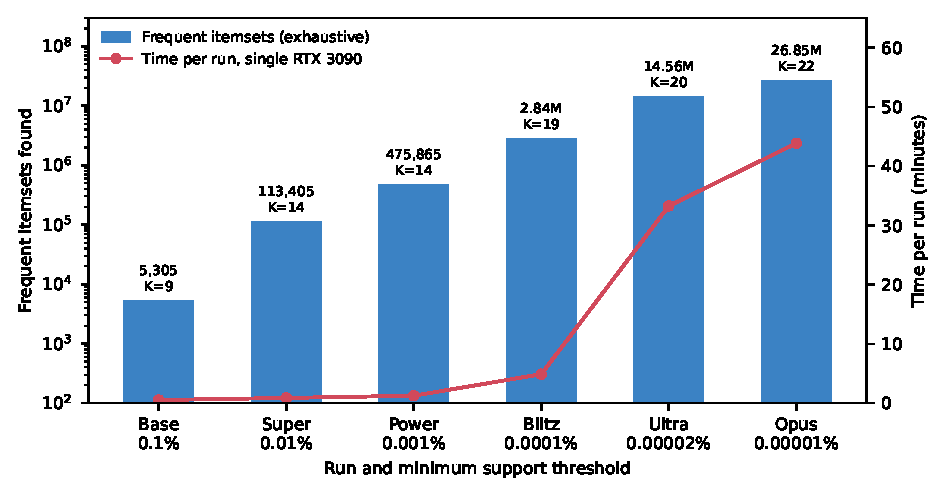
\includegraphics[width=\columnwidth]{figures/mining_campaign.pdf}
    \caption{Mining campaign across six support thresholds (exhaustive counts). Bars show frequent itemsets (log scale); line shows wall-clock time per run on a single RTX 3090.}
    \label{fig:campaign}
\end{figure}

\subsection{$K$-Distribution Analysis}

The Opus run reveals the complete $K$-distribution of protein feature co-occurrence (Figure~\ref{fig:kdist}, Table~\ref{tab:kdist}). The distribution is unimodal, peaking at $K{=}9$ with 3,529,257 itemsets (13.14\% of total), reflecting the interplay between combinatorial growth and support decay. The peak position is determined by the interaction between the item frequency distribution, the support threshold, and the co-occurrence structure of the data. Section~\ref{sec:null-model} demonstrates that this structure is biologically significant: a permutation-based null model that preserves per-protein feature counts while randomizing feature identities cannot produce patterns beyond $K{=}6$, confirming that the $K{=}9$ peak and all deeper patterns reflect genuine biological co-occurrence rather than statistical artifacts of annotation structure.

\begin{figure}[t]
    \centering
    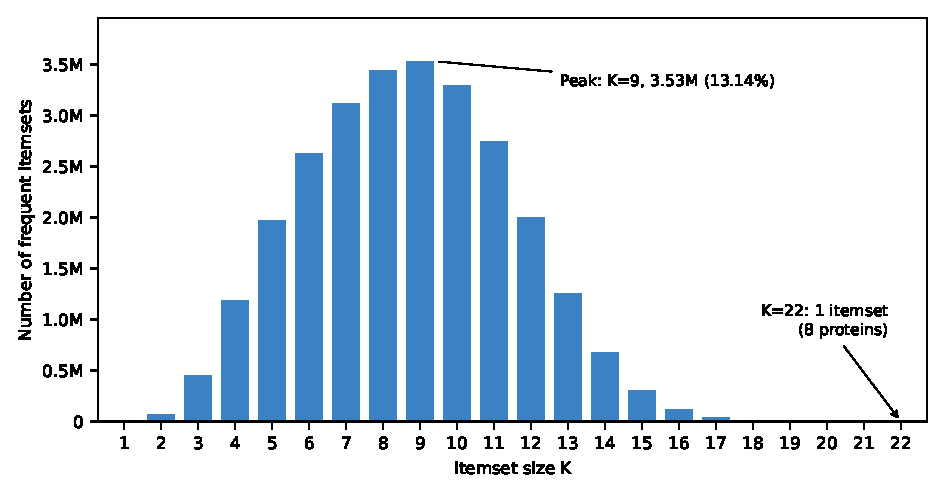
\includegraphics[width=\columnwidth]{figures/k_distribution.pdf}
    \caption{$K$-distribution of frequent itemsets at 0.00001\% support (26.8M total). The unimodal distribution peaks at $K{=}9$ (3.53M itemsets). A single itemset at maximum depth is shared by exactly 8 proteins.}
    \label{fig:kdist}
\end{figure}

\begin{table}[t]
\caption{$K$-distribution at 0.00001\% support (26.8M total).}
\label{tab:kdist}
\centering
\resizebox{\columnwidth}{!}{%
\footnotesize
\begin{tabular}{rrr|rrr}
\toprule
$K$ & Itemsets & \% & $K$ & Itemsets & \% \\
\midrule
1 & 1,002 & 0.00 & 12 & 1,996,772 & 7.44 \\
2 & 73,786 & 0.27 & 13 & 1,259,045 & 4.69 \\
3 & 452,777 & 1.69 & 14 & 679,471 & 2.53 \\
4 & 1,184,461 & 4.41 & 15 & 310,527 & 1.16 \\
5 & 1,974,126 & 7.35 & 16 & 118,659 & 0.44 \\
6 & 2,626,332 & 9.78 & 17 & 37,261 & 0.14 \\
7 & 3,118,459 & 11.61 & 18 & 9,375 & 0.03 \\
8 & 3,442,954 & 12.82 & 19 & 1,818 & 0.01 \\
\textbf{9} & \textbf{3,529,257} & \textbf{13.14} & 20 & 255 & $<\!$0.01 \\
10 & 3,293,612 & 12.27 & 21 & 23 & $<\!$0.01 \\
11 & 2,739,532 & 10.20 & 22 & 1 & $<\!$0.01 \\
\bottomrule
\end{tabular}%
}
\end{table}

\subsection{The $K{=}22$ Ceiling}

The single $K{=}22$ itemset is shared by exactly 8 proteins and comprises 22 co-occurring features (Table~\ref{tab:k22}).

\begin{table}[t]
\caption{$K{=}22$ itemset: 22 co-occurring features in 8 proteins.}
\label{tab:k22}
\centering
\resizebox{\columnwidth}{!}{%
\begin{tabular}{llp{4.2cm}}
\toprule
Category & ID & Description \\
\midrule
\multicolumn{3}{l}{\textit{Pfam domains (2)}} \\
& PF00270 & DEAD/DEAH helicase N-terminal \\
& PF00271 & Helicase C-terminal \\
\midrule
\multicolumn{3}{l}{\textit{Molecular Function (8)}} \\
& GO:0005524 & ATP binding \\
& GO:0016787 & Hydrolase activity \\
& GO:0000287 & Magnesium ion binding \\
& GO:0003697 & ssDNA binding \\
& GO:0003724 & RNA helicase activity \\
& GO:0003725 & dsRNA binding \\
& GO:0003678 & DNA helicase activity \\
& GO:0000978 & RNA Pol II regulatory binding \\
\midrule
\multicolumn{3}{l}{\textit{Biological Process (4)}} \\
& GO:0030154 & Cell differentiation \\
& GO:0045087 & Innate immune response \\
& GO:0051607 & Defense response to virus \\
& GO:0034605 & Cellular response to heat \\
\midrule
\multicolumn{3}{l}{\textit{Cellular Component (7)}} \\
& GO:0005737 & Cytoplasm \\
& GO:0005829 & Cytosol \\
& GO:0005634 & Nucleus \\
& GO:0005739 & Mitochondrion \\
& GO:0030424 & Axon \\
& GO:0030425 & Dendrite \\
& GO:0016607 & Nuclear speckle \\
\midrule
\multicolumn{3}{l}{\textit{Structural property (1)}} \\
& plddt\_mean\_med & Medium confidence (mean pLDDT 50--90) \\
\bottomrule
\end{tabular}%
}
\end{table}

This 22-feature signature is \emph{consistent with} a neuronal antiviral RNA-helicase profile---a DEAD/DEAH-box helicase with dual RNA/DNA unwinding annotations, innate-immune annotations, and simultaneous annotation across multiple cellular compartments including axons, dendrites, nuclear speckles, and mitochondria. DEAD-box helicases such as RIG-I and MDA5 are established viral RNA sensors in innate immunity~\cite{rehwinkel2020}, so this configuration is biologically plausible; we emphasise, however, that it is a co-occurrence of annotations, not a demonstrated mechanism (Section~\ref{sec:discussion}). The 22 features contain \emph{no} GO parent--child pairs, so the depth is not an artifact of the GO true-path rule; the single definitional link is GO:0005524 (ATP binding), which InterPro2GO derives from PF00270 (InterPro IPR011545; PF00271/IPR001650 carries no GO mapping, and neither entry maps to any other member), leaving 21 independently annotated features. The eight matching proteins were identified with \texttt{analyze\_k22\_proteins.py}; their accessions are deposited with the run artifacts (see Data and Code Availability), and the full transaction matrix is regenerable from the source UniProt release via the released feature-extraction pipeline.

This ceiling is not an artifact of insufficient computational depth. Each of the 8 proteins possesses \emph{exactly} 22 annotated features in our vocabulary, so this particular itemset cannot be extended. The ceiling itself is empirical rather than structural: the vocabulary places up to 46 features on a single protein, but only 32 of the 76.9 million mined proteins carry 22 or more features and only 19 carry 23 or more. A $K{=}23$ itemset would require at least $\text{min\_count}$ of those 19 proteins to share the same 23 features. None do at the Opus threshold, and lowering the threshold to 4 proteins (48,007,493 itemsets; 75.6\,min on 2$\times$RTX 3090) still terminates at $K{=}22$, with 342 itemsets at $K{=}20$, 27 at $K{=}21$ and the same single itemset at $K{=}22$.

\subsection{Biological Discoveries at Intermediate $K$-Levels}

Beyond the maximum depth, the mining campaign reveals conserved molecular machines. We highlight five intermediate patterns, selected to span distinct $K$-levels and biological systems. We prioritized patterns with known experimental validation (established drug targets, characterized molecular machines) to demonstrate that the mining recovers known biology:

\paragraph{$K{=}19$: RNA Spliceosome Processing Hub} (187 proteins). DEAD/DEAH-box helicases linked with RNA splicing, mRNA processing, nucleolus localization, and translation regulation, the core pre-mRNA splicing machinery~\cite{wahl2009}.

\paragraph{$K{=}17$: Receptor Tyrosine Kinase Signaling Hub}
(${\sim}611$ proteins). Protein tyrosine kinase (PF07714) with SH2 (PF00017)
and SH3 (PF00018) adaptor domains---the canonical Src-family kinase
architecture~\cite{boggon2004}---co-occurring with intracellular signal transduction, DNA repair,
apoptosis, oxidative stress response, cell adhesion, actin binding, and gene
regulation. This 17-feature combination describes the core receptor tyrosine
kinase (RTK) signaling machinery, one of the most targeted pathways in cancer
drug discovery: imatinib, dasatinib, and erlotinib all target proteins matching
this functional signature.

\paragraph{$K{=}13$: Helicase-Recombinase DNA Repair Module} (itemsets at this level are shared by up to 11,521 proteins\footnote{Supporting-protein counts are read from the per-$K$ itemset tables of the Blitz run. Where the pattern is identified by named domains, the count is the support of the matching itemsets; the $K{=}13$ and $K{=}11$ descriptions name no domain identifiers, so the maximum support at that level is given instead.}). DEAD-box helicases co-occurring with DNA repair, recombination, replication, and the SOS response, consistent with bacterial RecBCD-like repair complexes~\cite{dillingham2008}, recovered here from annotation data alone.

\paragraph{$K{=}12$: Bacterial Cell Wall Synthase} (up to 16,185 proteins; 111 itemsets at this level contain both domains). Penicillin-binding protein domains (PF00905 transpeptidase, PF00912 transglycosylase) with cell wall organization and peptidoglycan biosynthesis~\cite{sauvage2008}. This is a \emph{validated drug target}: beta-lactam antibiotics bind these exact domains. ET-miner recovered this known target from annotation data alone, without manual target selection, validating that the mining captures established biology.

\paragraph{$K{=}11$: AAA+ ATPase Proteasome Complex} (up to 28,913 proteins). Protein quality control machinery: AAA-family ATPase with Clp protease domains. The bacterial equivalent of the eukaryotic ubiquitin-proteasome system.

\subsection{Statistical Validation: Null Model}
\label{sec:null-model}

To test whether the observed $K$-distribution reflects genuine biological co-occurrence or arises from marginal feature frequencies alone, we performed a permutation-based null model analysis. For each permutation, all transactions were exploded into (protein, feature) pairs, a Fisher--Yates shuffle was applied to the feature column---preserving per-protein feature counts---and duplicate features within each protein were removed (so per-protein counts are preserved up to those removals) before re-mining at the 0.001\% support threshold ($\text{min\_count}{=}769$). One hundred permutations were run (seed~42) in 2,007\,s wall-clock on the two RTX 3090s with the row-split path (18.6\,s per permutation).

Table~\ref{tab:null-model} compares the biological and null $K$-distributions. The null model peaks at $K{=}3$ (46.2\% of null itemsets) and generates between 19 and 25 itemsets at $K{=}6$ (mean 21.7); no permutation produced any pattern at $K{\geq}7$. In contrast, the biological data contains 88,745 itemsets at $K{\geq}7$ and extends to $K{=}14$.

\begin{table}[t]
\caption{Biological vs.\ null model $K$-distributions at 0.001\% support (100 permutations, seed 42). $Z=(\text{Bio}-\mu)/\sigma$ with $\mu$ and $\sigma$ estimated from the 100 permutations; because $\sigma$ is tiny relative to the biological excess, the magnitudes indicate strong enrichment rather than calibrated tail probabilities. $p$ is the one-sided empirical permutation $p$-value for enrichment with the $+1$ correction~\cite{phipson2010}, whose resolution with 100 permutations is $1/101{\approx}0.0099$. $K{\geq}7$ patterns are absent from all 100 null runs; the exact one-sided binomial 95\% upper bound on the per-permutation probability of any such pattern is $1-0.05^{1/100}=0.0295$.}
\label{tab:null-model}
\centering
\resizebox{\columnwidth}{!}{%
\small
\begin{tabular}{rrrrrrl}
\toprule
$K$ & Bio & Null $\mu$ & Null $\sigma$ & $Z$ & $p$ & \\
\midrule
1 & 1,002 & 1,002 & 0.0 & 0.0 & 1.0 & preserved \\
2 & 22,019 & 63,703 & 33.6 & $-1{,}239$ & 1.0 & depleted \\
3 & 73,205 & 79,144 & 46.5 & $-128$ & 1.0 & depleted \\
4 & 108,059 & 25,442 & 30.3 & $+2{,}728$ & 0.0099 & enriched \\
5 & 104,239 & 1,993 & 9.6 & $+10{,}632$ & 0.0099 & enriched \\
6 & 78,596 & 21.7 & 1.1 & $+68{,}730$ & 0.0099 & enriched \\
7--14 & 88,745 & 0 & 0.0 & --- & 0.0099 & enriched \\
\bottomrule
\end{tabular}%
}
\end{table}

Three findings emerge. First, $K{=}2$ and $K{=}3$ patterns are \emph{depleted} in biological data relative to the null ($Z{=}{-}1{,}239$ and ${-}128$, respectively): random shuffling of common features produces more frequent pairs and triples than biology, because evolution assembles features into specific functional modules rather than combining them promiscuously. Second, for $K{\geq}4$, biological co-occurrence massively exceeds the null expectation (standardized effect sizes of $+2{,}728$ at $K{=}4$, $+10{,}632$ at $K{=}5$ and $+68{,}730$ at $K{=}6$); with 100 permutations the empirical $p$-value of every enriched level is at its resolution limit, $p{=}1/101{\approx}0.0099$~\cite{phipson2010}. Third, in 0 of 100 permutations did the null model produce itemsets beyond $K{=}6$; the exact one-sided binomial 95\% upper bound on the per-permutation probability of any $K{\geq}7$ itemset is $1-0.05^{1/100}{=}0.0295$. Random co-occurrence therefore cannot produce deep feature combinations at this threshold.

The $K{=}1$ row confirms that all 1,002 features remain frequent after shuffling, verifying that every item stays frequent under the shuffle. This null model directly validates significance at the 0.001\% support level ($\text{min\_count}{=}769$); the biological reference is the exhaustive Direct CSR$\to$GPU mining at this threshold (475,865 itemsets, reaching $K{=}14$), i.e.\ the Power row of Table~\ref{tab:campaign}. The Opus threshold results ($\text{min\_count}{=}8$, $K_\text{max}{=}22$, Table~\ref{tab:kdist}) were obtained at a more permissive threshold where a separate null model was not run; a rigorous statistical claim at that threshold would require its own permutation analysis.

%==============================================================================
\section{Discussion}
\label{sec:discussion}
%==============================================================================

\subsection{Computational Significance}

ET-miner demonstrates that exact Apriori computation is feasible at the 100-million-transaction scale on a single consumer GPU. The full-set $206\text{\,GB}$ dense matrix, the $5.1\text{\,GB}$ coordinate-format sparse matrix of the mined subset, and its $9.6\text{\,GB}$ GPU bitvector matrix ($26\text{\,GB}$ for the full set) illustrate a compression path applicable to any sparse, high-dimensional transaction dataset (the same-subset dense-to-CSR reduction is ${\sim}15\times$). The GPU-resident bitvector architecture is critical: bitvectors stay on-GPU across all 22 iterations, with only lightweight metadata (prefix groups and result indices) crossing the PCIe bus, versus full candidate and support array transfers in conventional approaches.

The comparison between the streaming SON path and the Direct CSR$\to$GPU path (Section~\ref{sec:results}) shows that the price of streaming is time, not completeness: at identical support (0.001\%) the released SON implementation returns the same itemset count and $K$-distribution as the exhaustive run, but $99\times$ more slowly (6,151.1\,s vs.\ 62.2\,s on the RTX 3090): its chunk-local mining pass took 88\,minutes for the two chunks and the global re-counting pass a further 14\,minutes. A two-pass SON with a proportional or lowered local threshold cannot miss a globally frequent itemset~\cite{savasere1995}.

\subsection{Comparison with Prior GPU FIM Systems}

Several GPU-accelerated FIM systems have been proposed (Table~\ref{tab:scale-comparison}). GPApriori~\cite{zhang2011} achieved up to $100\times$ speedup on FIMI benchmarks using static bitsets. GMiner~\cite{chon2018} introduced streaming of transaction bitmap chunks to the GPU with overlapping data transfer and computation. GMiner++~\cite{chon2024} reduced redundant computation through pre-calculated bit arrays. CGSS~\cite{djenouri2019} combined GPU and cluster computing. BIGMiner~\cite{chon2018b} achieved the largest prior scale at 100M transactions on 30 MapReduce nodes. Fang et al.~\cite{fang2009} established the foundational GPU-FIM architecture. A comprehensive survey by Bustio-Mart\'inez et al.~\cite{acmsurvey2021} confirms that Apriori-based approaches dominate GPU implementations due to their regular, level-wise structure. For a systematic review of FIM in bioinformatics, see Naulaerts et al.~\cite{naulaerts2015}. All prior systems share two fundamental limitations: (1)~they store the database as a dense bitmap that must be repeatedly transferred between CPU and GPU memory, and (2)~they were evaluated on datasets of at most a few million real transactions, one to two orders of magnitude smaller than our proteome dataset.

\begin{table}[t]
\caption{Scale comparison of GPU and distributed FIM systems. ET-miner processes $5.1\times$ more transactions than the largest prior single-machine GPU system (GMiner, 15M synthetic transactions; 1.7M real) and mines exhaustively to $K{=}22$, deeper than any previously reported GPU FIM result.}
\label{tab:scale-comparison}
\centering
\resizebox{\columnwidth}{!}{%
\small
\begin{tabular}{@{}lrrrll@{}}
\toprule
\textbf{System} & \textbf{Transactions} & \textbf{Items} & \textbf{Max $K$} & \textbf{Hardware} & \textbf{Time} \\
\midrule
Borgelt~\cite{borgelt2003} & 100K & 500 & $\sim$10 & 1$\times$ CPU & 1--100\,s \\
Fang~\cite{fang2009} & 100K & 1K & $\sim$5 & 1$\times$ GTX 280 & 1--10\,s \\
GMiner~\cite{chon2018} & 15M & 20K & $\sim$30 & 4$\times$ GTX 1080 & 20--150\,s \\
BIGMiner~\cite{chon2018b} & 100M & 100K & --- & 30$\times$ servers & 1--20K\,s \\
\midrule
ET-miner & \textbf{76.9M} & 1,002 & \textbf{22} & 1$\times$ RTX 3090 & 43.9\,min \\
\bottomrule
\end{tabular}%
}
\end{table}

The key difference is straightforward: existing GPU mining systems generate
candidates on the CPU and repeatedly stream data between CPU and GPU memory;
ET-miner loads the data onto the GPU once and never moves it back.

ET-miner's design eliminates these bottlenecks through three key choices:

\begin{enumerate}[leftmargin=*,itemsep=2pt]

\item \textbf{Sparse encoding, dense computation.}
The transaction database is stored in compressed sparse format (CSR), transferred to the GPU once (${\sim}3.1$\,GB of CSR arrays versus 9.6\,GB for the equivalent bit-packed dense bitmap of the 76.9M mining subset, a saving that grows with sparsity; see Table~\ref{tab:memory-comparison}), and expanded into a column-oriented bitvector matrix directly on the GPU. Prior systems transfer the full dense matrix at every mining iteration.

\item \textbf{GPU-accelerated mining loop.}
Once the bitvector matrix is built on-GPU, candidate generation, support counting and threshold filtering execute on the device without touching the database again. The per-iteration communication is limited to the prefix-group arrays of the previous level (uploaded) and the surviving (index, count) records of the current level (downloaded, 12\,bytes each), both proportional to the number of frequent itemsets rather than to the database. In contrast, GMiner's cost model~\cite{chon2018} identifies repeated CPU--GPU data streaming as the dominant and irreducible performance bottleneck.

\item \textbf{Automatic multi-GPU scaling.}
For candidate spaces exceeding a single device, ET-miner can distribute work across multiple GPUs either by candidate index or by row split, the latter with chunk sizing measured from the installed VRAM. The mining campaign of Table~\ref{tab:campaign} used a single RTX 3090, and the 76.9M multi-feature proteins were mined without manual tuning; the row-split two-GPU path was used for the per-level itemset exports and the null model.

\end{enumerate}

\noindent For readers interested in GPU implementation details, a detailed kernel-level comparison (candidate generation strategy, popcount width, reduction hierarchy, per-stage execution location, and memory footprint analysis) is provided in Appendix~\ref{app:gpu-comparison}.

\subsection{Comparison with Protein Domain Mining}

Prior protein domain co-occurrence studies are fundamentally limited in scope. Wang et al.~\cite{wang2011} constructed Domain Co-occurrence Networks revealing scale-free properties, but this approach is inherently pairwise ($K{=}2$) and limited to individual proteomes. Terrapon et al.~\cite{coin2009} used statistical co-occurrence for novel domain detection in \emph{Plasmodium falciparum}, again limited to pairs. Meysman et al.~\cite{meysman2015} mined spatially cohesive amino acid patterns from the PDB, but addressed 3D proximity rather than domain-level combinations and was limited to ${\sim}32$K structures. Mrzic et al.~\cite{mrzic2018} reviewed frequent subgraph mining for biomolecular data, noting that graph mining is NP-hard and scales poorly.

None of these approaches perform exhaustive itemset mining beyond $K{=}2$. ET-miner's discovery of patterns spanning up to 22 co-occurring features across the full AlphaFold universe~\cite{varadi2024} represents a qualitative advance. The Encyclopedia of Domains~\cite{barrio2024} catalogs individual domains across the database; ET-miner complements it by discovering which domain \emph{combinations} co-occur, the higher-order patterns that individual domain analysis cannot reveal.

\subsection{Biological Significance}

The $K{=}22$ neuronal antiviral sentinel combines four distinct functional roles: (1)~RNA/DNA unwinding, (2)~innate immune sensing, (3)~gene regulation, and (4)~neuronal function. The multi-compartment localization (simultaneous presence in axons, dendrites, nuclear speckles, and mitochondria) suggests these proteins may function as pre-positioned immune sensors, enabling rapid local response to viral invasion across the neuron's spatial extent. However, this interpretation should be treated as a hypothesis rather than an established mechanism: the co-occurrence of these 22 annotations does not by itself demonstrate functional coupling. Moreover, annotation completeness varies substantially across organisms: well-studied model organisms (human, mouse, \emph{E.~coli}) have far richer GO annotations than poorly characterized taxa, which could inflate apparent $K$ values for proteins from these organisms. The $K{=}22$ ceiling reflects the depth of current UniProt annotations rather than a fundamental limit of biological complexity; future annotation campaigns may reveal deeper co-occurrence patterns.

The unimodal peak at $K{=}9$ (3.53 million itemsets, 13.14\% of all patterns) occurs where combinatorial growth and support decay intersect. The permutation-based null model (Section~\ref{sec:null-model}) confirms that this peak reflects genuine biological modularity rather than a statistical artifact: random shuffling cannot produce any patterns at $K{\geq}7$, and even at $K{=}4$ the biological count exceeds the null expectation $4.2$-fold (108,059 vs.\ 25,442; a standardized effect size of $+2{,}728$ estimated from 100 permutations). This is consistent with the modular architecture of protein functional domains~\cite{chothia2003}, where evolution reuses and combines a finite set of building blocks into increasingly specific functional configurations.

At intermediate $K$-levels, ET-miner recovers known biology with increasing specificity. The $K{=}12$ bacterial cell wall synthase module (Section~\ref{sec:results}) validates the approach: beta-lactam antibiotics target these exact domain combinations, yet ET-miner recovered this co-occurrence pattern from annotation data alone, without manual target selection. The five highlighted patterns ($K{=}11$ to $K{=}19$) were selected to illustrate the diversity of function across the $K$-distribution, not as an exhaustive catalog.

These biological interpretations carry important caveats: electronically propagated GO annotations may create artificial co-occurrence~\cite{rhee2008}, and many itemsets are subsets or supersets of each other. However, the null model analysis (Section~\ref{sec:null-model}) demonstrates that the higher-order patterns ($K{\geq}4$) cannot be explained by annotation structure alone. We discuss additional methodological limitations in Section~\ref{sec:limitations}.

\subsection{Limitations and Future Work}
\label{sec:limitations}

\setlength{\parindent}{0pt}%
Several methodological limitations should be noted.

\textbf{1.}~Our null model analysis (Section~\ref{sec:null-model}) validates the $K$-distribution at the aggregate level but does not test whether \emph{individual} itemsets are statistically significant. Established frameworks for statistically significant pattern discovery~\cite{webb2007,webb2014} could be adapted here: a per-itemset significance test would require comparing each pattern's observed support against its expected support under the null, with false discovery rate correction for the millions of patterns tested. Such pattern-level testing would enable prioritization of the most surprising co-occurrences for experimental follow-up.

\textbf{2.}~The Gene Ontology's true-path rule guarantees that any protein annotated with a specific GO term is also annotated with all parent terms, creating structured co-occurrence that is definitional rather than biological. This inflates itemset counts and $K$ values in ways that do not reflect independent functional coupling. We note, however, that the deepest ($K{=}22$) itemset contains 0 parent--child pairs, so its depth is not driven by this effect (Section~\ref{sec:results}).

\textbf{3.}~GO annotations are updated monthly; our results reflect UniProt TrEMBL release 2026\_01 and may vary with different releases (see Section~\ref{sec:methods}).

\textbf{4.}~Our analysis excludes 128.7 million proteins (62.6\%) with only a single annotated feature. This exclusion biases toward well-annotated organisms and proteins, potentially underrepresenting poorly studied taxa.

\textbf{5.}~Many of the discovered patterns are subsets or supersets of each other. ET-miner implements closed itemset filtering as a post-processing step: after each $K$-level's support counting is complete, non-closed itemsets (those whose support equals that of a proper superset) are removed. We report the complete pattern space here to characterize the full $K$-distribution. Filtering to closed or maximal frequent itemsets would substantially reduce redundancy and is recommended for downstream biological analysis.

\subsubsection*{AlphaFold Complex Structures}

The AlphaFold database has recently expanded to include predicted protein complexes~\cite{abramson2024}: 1.7 million high-confidence homodimer predictions have been added to the database, with an additional 18 million lower-confidence homodimers available via bulk download. Heterodimer predictions are being assessed and will follow. This expansion---described as ``a first step towards a comprehensive description of the human interactome'' (EMBL-EBI, 2026)---directly motivates extending ET-miner to protein-protein interactions. Each chain in a complex can be treated as a separate transaction with shared features, or the complex itself can serve as the transaction unit with interaction-derived features (interface contacts, buried surface area, chain stoichiometry) added to the vocabulary. Mining conserved interaction motifs---patterns of features that co-occur specifically in the context of protein complexes---could reveal allosteric coupling and assembly dependencies invisible to monomer-level analysis, with direct relevance for therapeutic design and understanding host-pathogen interactions.

The most promising future direction is incorporating structure-derived features from AlphaFold's predicted 3D coordinates (inter-residue contact maps, binding pocket geometry, and pharmacophoric features), which could reveal conserved 3D functional architectures invisible to annotation-based analysis and directly connect to drug discovery through pharmacophore-level pattern mining.
\setlength{\parindent}{1em}%

%==============================================================================
\section{Conclusion}
\label{sec:conclusion}
%==============================================================================

ET-miner demonstrates that exhaustive frequent itemset mining at the 100-million-transaction scale is practical on a single consumer GPU. With a base vocabulary of 1,002 features on one NVIDIA GeForce RTX 3090, mining completes in 43.9 minutes (excluding the one-time feature extraction, Section~\ref{sec:methods}) and reaches $K{=}22$.

A permutation-based null model at the Power threshold supports biological significance: in 100 permutations preserving per-protein feature counts, no null run reached $K{\geq}7$ (empirical $p{\approx}0.01$), against 88,745 biological itemsets at $K{\geq}7$ (Section~\ref{sec:null-model}). The resulting patterns provide the first systematic map of higher-order protein functional modularity across the entire known protein universe---architecture that no pairwise analysis could reveal. As the AlphaFold database expands to protein complexes and structure-derived features, ET-miner's architecture positions it to mine the next generation of structural proteomics data without architectural changes.

A preprint of this work is archived at Zenodo (DOI: \texttt{10.5281/zenodo.18674353}). Source code and mining results will be released as open-source software upon publication at \url{https://github.com/Et9797/ET-miner}.

\subsection*{Author Information}
\small
\begin{tabular}{@{}ll@{}}
E.\ Ahmic & Indep. Researcher (MSc. Drug Innovation, UU) \\
\end{tabular}

\smallskip
\noindent Correspondence to E.\ Ahmic. \ \texttt{etet1997@hotmail.com}
\normalsize

\subsection*{Funding}
\small
\noindent This research received no external funding. Computations were run on a rented vast.ai cloud instance with two NVIDIA GeForce RTX 3090 GPUs.
\normalsize

\subsection*{Competing Interests}
\small
\noindent The authors declare no competing financial interests. Claude Code is affiliated with Anthropic; E.\ Ahmic is an independent researcher with no affiliation with, or financial interest in Anthropic.
\normalsize

\subsection*{Ethics}
\small
\noindent This study used only publicly available protein sequence and structure data (UniProt and the AlphaFold Protein Structure Database) and involved no human or animal subjects.
\normalsize

\subsection*{Data and Code Availability}
\small
\noindent The mining source code, the feature-extraction pipeline, and the summary result artefacts (per-run mining logs, $K$-distribution tables, null-model outputs, and the feature-to-item mapping) will be released at \url{https://github.com/Et9797/ET-miner} upon publication. This manuscript is a revised version of the preprint archived at Zenodo (DOI \texttt{10.5281/zenodo.18674353}). The full intermediate transaction matrix is not deposited owing to its size; it is regenerable from UniProt TrEMBL release 2026\_01 (archived under \texttt{previous\_releases} on the UniProt FTP site) via the released feature-extraction pipeline. The complete run that produced every value in this paper (scripts, logs, per-$K$ itemset tables, null-model outputs, the accessions of the $K{=}22$ proteins and a per-claim comparison against the preprint) is deposited in the same repository under \texttt{runs/20260902T0000Z/}. The values of the preprint that this version supersedes (hardware, timings, streaming-path counts and five-permutation statistics) are itemized in \texttt{COMPARISON\_REPORT.md} at the repository root.
\normalsize

%==============================================================================
% References
%==============================================================================

\bibliographystyle{unsrt}

\begin{thebibliography}{38}

\bibitem{jumper2021}
J.~Jumper et al.
\newblock Highly accurate protein structure prediction with AlphaFold.
\newblock \emph{Nature}, 596:583--589, 2021.

\bibitem{varadi2022}
M.~Varadi et al.
\newblock AlphaFold Protein Structure Database: massively expanding the structural coverage of protein-sequence space with high-accuracy models.
\newblock \emph{Nucleic Acids Research}, 50(D1):D439--D444, 2022.

\bibitem{wang2011}
Z.~Wang, X.-C.~Zhang, M.~H.~Le, D.~Xu, G.~Stacey, and J.~Cheng.
\newblock A protein domain co-occurrence network approach for predicting protein function and inferring species phylogeny.
\newblock \emph{PLoS ONE}, 6(3):e17906, 2011.

\bibitem{coin2009}
N.~Terrapon et al.
\newblock Detection of new protein domains using co-occurrence: application to \emph{Plasmodium falciparum}.
\newblock \emph{Bioinformatics}, 25(23):3077--3083, 2009.

\bibitem{meysman2015}
P.~Meysman, C.~Zhou, B.~Cule, B.~Goethals, and K.~Laukens.
\newblock Mining the entire Protein DataBank for frequent spatially cohesive amino acid patterns.
\newblock \emph{BioData Mining}, 8:4, 2015.

\bibitem{agrawal1994}
R.~Agrawal and R.~Srikant.
\newblock Fast algorithms for mining association rules in large databases.
\newblock In \emph{Proc.\ 20th Int.\ Conf.\ Very Large Data Bases (VLDB)}, pp.\ 487--499, 1994.

\bibitem{luna2019}
J.~M.~Luna, P.~Fournier-Viger, and S.~Ventura.
\newblock Frequent itemset mining: A 25 years review.
\newblock \emph{WIREs Data Mining and Knowledge Discovery}, 9(6), 2019.

\bibitem{han2000}
J.~Han, J.~Pei, and Y.~Yin.
\newblock Mining frequent patterns without candidate generation.
\newblock In \emph{Proc.\ ACM SIGMOD}, pp.\ 1--12, 2000.

\bibitem{zaki2000}
M.~J.~Zaki.
\newblock Scalable algorithms for association mining.
\newblock \emph{IEEE Trans.\ Knowledge and Data Engineering}, 12(3):372--390, 2000.

\bibitem{zhang2011}
F.~Zhang, Y.~Zhang, and J.~Bakos.
\newblock GPApriori: GPU-accelerated frequent itemset mining.
\newblock In \emph{Proc.\ IEEE Int.\ Conf.\ Cluster Computing}, pp.\ 590--594, 2011.

\bibitem{chon2018}
K.-W.~Chon, S.-H.~Hwang, and M.-S.~Kim.
\newblock GMiner: A fast GPU-based frequent itemset mining method for large-scale data.
\newblock \emph{Information Sciences}, 439--440:19--38, 2018.

\bibitem{djenouri2019}
Y.~Djenouri et al.
\newblock CGSS: Combined GPU-Cluster single scan for frequent itemset mining.
\newblock \emph{Information Sciences}, 496:363--377, 2019.

\bibitem{acmsurvey2021}
L.~Bustio-Mart\'inez, R.~Cumplido, M.~Letras, R.~Hern\'andez-Le\'on, C.~Feregrino-Uribe, and J.~Hern\'andez-Palancar.
\newblock FPGA/GPU-based acceleration for frequent itemset mining: A comprehensive review.
\newblock \emph{ACM Computing Surveys}, 54(9):179:1--179:35, 2021.

\bibitem{varadi2024}
M.~Varadi et al.
\newblock AlphaFold Protein Structure Database in 2024.
\newblock \emph{Nucleic Acids Research}, 52(D1):D368--D375, 2024.

\bibitem{savasere1995}
A.~Savasere, E.~Omiecinski, and S.~Navathe.
\newblock An efficient algorithm for mining association rules in large databases.
\newblock In \emph{Proc.\ 21st VLDB Conf.}, pp.\ 432--444, 1995.

\bibitem{chon2024}
K.-W.~Chon et al.
\newblock Boosting GPU-based frequent itemset mining by reducing redundant computations.
\newblock \emph{Expert Systems with Applications}, 250:123928, 2024.

\bibitem{mrzic2018}
A.~Mrzic, P.~Meysman, W.~Bittremieux, P.~Moris, B.~Cule, B.~Goethals, and K.~Laukens.
\newblock Grasping frequent subgraph mining for bioinformatics applications.
\newblock \emph{BioData Mining}, 11:20, 2018.

\bibitem{barrio2024}
A.~M.~Lau et al.
\newblock Exploring structural diversity across the protein universe with The Encyclopedia of Domains.
\newblock \emph{Science}, 386(6721):eadq4946, 2024.

\bibitem{rehwinkel2020}
J.~Rehwinkel and M.~U.~Gack.
\newblock RIG-I-like receptors: their regulation and roles in RNA sensing.
\newblock \emph{Nature Reviews Immunology}, 20(9):537--551, 2020.

\bibitem{chothia2003}
C.~Chothia, J.~Gough, C.~Vogel, and S.~A.~Teichmann.
\newblock Evolution of the protein repertoire.
\newblock \emph{Science}, 300(5626):1701--1703, 2003.

\bibitem{boggon2004}
T.~J.~Boggon and M.~J.~Eck.
\newblock Structure and regulation of Src family kinases.
\newblock \emph{Oncogene}, 23(48):7918--7927, 2004.

\bibitem{sauvage2008}
E.~Sauvage, F.~Kerff, M.~Terrak, J.~A.~Ayala, and P.~Charlier.
\newblock The penicillin-binding proteins: structure and role in peptidoglycan biosynthesis.
\newblock \emph{FEMS Microbiology Reviews}, 32(2):234--258, 2008.

\bibitem{rhee2008}
S.~Y.~Rhee, V.~Wood, K.~Dolinski, and S.~Draghici.
\newblock Use and misuse of the gene ontology annotations.
\newblock \emph{Nature Reviews Genetics}, 9(7):509--515, 2008.

\bibitem{wahl2009}
M.~C.~Wahl, C.~L.~Will, and R.~L\"uhrmann.
\newblock The spliceosome: design principles of a dynamic RNP machine.
\newblock \emph{Cell}, 136(4):701--718, 2009.

\bibitem{dillingham2008}
M.~S.~Dillingham and S.~C.~Kowalczykowski.
\newblock RecBCD enzyme and the repair of double-stranded DNA breaks.
\newblock \emph{Microbiology and Molecular Biology Reviews}, 72(4):642--671, 2008.

\bibitem{uniprot2023}
The UniProt Consortium.
\newblock UniProt: the Universal Protein Knowledgebase in 2023.
\newblock \emph{Nucleic Acids Research}, 51(D1):D523--D531, 2023.

\bibitem{go2023}
Gene Ontology Consortium.
\newblock The Gene Ontology knowledgebase in 2023.
\newblock \emph{Genetics}, 224(1):iyad031, 2023.

\bibitem{mistry2021}
J.~Mistry et al.
\newblock Pfam: The protein families database in 2021.
\newblock \emph{Nucleic Acids Research}, 49(D1):D412--D419, 2021.

\bibitem{naulaerts2015}
S.~Naulaerts, P.~Meysman, W.~Bittremieux, T.~N.~Vu, W.~Vanden~Berghe, B.~Goethals, and K.~Laukens.
\newblock A primer to frequent itemset mining for bioinformatics.
\newblock \emph{Briefings in Bioinformatics}, 16(2):216--231, 2015.

\bibitem{fang2009}
W.~Fang, K.~K.~Lau, M.~Lu, X.~Xiao, C.~K.~Lam, P.~Y.~Yang, B.~He, Q.~Luo, P.~V.~Sander, and K.~Yang.
\newblock Frequent itemset mining on graphics processors.
\newblock In \emph{Proc.\ DaMoN Workshop}, pp.\ 34--42, 2009.

\bibitem{webb2007}
G.~I.~Webb.
\newblock Discovering significant patterns.
\newblock \emph{Machine Learning}, 68(1):1--33, 2007.

\bibitem{webb2014}
G.~I.~Webb and J.~Vreeken.
\newblock Efficient discovery of the most interesting associations.
\newblock \emph{ACM Trans.\ Knowledge Discovery from Data}, 8(3):15, 2014.

\bibitem{abramson2024}
J.~Abramson et al.
\newblock Accurate structure prediction of biomolecular interactions with AlphaFold~3.
\newblock \emph{Nature}, 630:493--500, 2024.

\bibitem{chon2018b}
K.-W.~Chon and M.-S.~Kim.
\newblock BIGMiner: A fast and scalable distributed frequent pattern miner for big data.
\newblock \emph{Cluster Computing}, 21(3):1507--1520, 2018.

\bibitem{borgelt2003}
C.~Borgelt.
\newblock Efficient implementations of Apriori and Eclat.
\newblock In \emph{Proc.\ FIMI Workshop}, CEUR-WS Vol.~90, 2003.

\bibitem{zaki1997}
M.~J.~Zaki, S.~Parthasarathy, M.~Ogihara, and W.~Li.
\newblock New algorithms for fast discovery of association rules.
\newblock In \emph{Proc.\ 3rd Int.\ Conf.\ Knowledge Discovery and Data Mining (KDD)}, pp.\ 283--296, 1997.

\bibitem{phipson2010}
B.~Phipson and G.~K.~Smyth.
\newblock Permutation $p$-values should never be zero: calculating exact $p$-values when permutations are randomly drawn.
\newblock \emph{Statistical Applications in Genetics and Molecular Biology}, 9(1):39, 2010.

\bibitem{miettinen2020}
P.~Miettinen and S.~Neumann.
\newblock Recent developments in Boolean matrix factorization.
\newblock In \emph{Proc.\ IJCAI Survey Track}, pp.\ 4922--4928, 2020.

\end{thebibliography}

%==============================================================================
\clearpage
\appendix
\onecolumn

\begin{center}
{\Large\bfseries Appendix}
\end{center}
\vspace{0.5em}
\hrule
\vspace{1.5em}

\section{Complexity Analysis}
\label{app:complexity}
%==============================================================================

The bitvector representation processes 64 proteins per CPU/GPU operation, providing a $64\times$ constant-factor speedup over na\"ive element-wise comparison. GPU parallelism amplifies this further.

\paragraph{Space complexity.}
CPU: $O(\text{nnz})$ for CSR construction (temporary). GPU: $O(|F_1| \times \lceil N/64 \rceil)$ for bitvectors (persistent across all $K$-levels), plus $O(|F_k|)$ per level for intermediate results.

\paragraph{Time complexity per $K$-level.}
$K{=}1$: $O(|F_1| \times \lceil N/64 \rceil / P)$, where $P$ is GPU thread parallelism.
$K{=}2$: $O(\binom{|F_1|}{2} \times \lceil N/64 \rceil / P)$.
$K{\geq}k$: $O(|\text{candidates}_k| \times k \times \lceil N/64 \rceil / P)$.

The bitvector approach reduces support counting from $O(N)$ integer comparisons to $O(\lceil N/64 \rceil)$ bitwise AND + popcount operations---a $64\times$ constant factor improvement, further amplified by GPU SIMD parallelism.

%==============================================================================
\section{Algorithm Pseudocode}
\label{app:pseudocode}
%==============================================================================

\begin{algorithm}[H]
\caption{ET-miner GPU-Accelerated Apriori}
\label{alg:etminer}
\begin{algorithmic}[1]
\Require Transactions $T$ (Parquet), minimum support $\sigma$
\Ensure Frequent itemsets $F$ with support values
\State $n \gets |T|$; $\text{min\_count} \gets \lceil \sigma \cdot n \rceil$
\State $F_1 \gets \{i : \text{count}(i) \geq \text{min\_count}\}$ \Comment{Streaming}
\State $\text{CSR} \gets \text{BuildCSR}(T, F_1)$ \Comment{$O(\text{nnz})$ memory}
\State $B \gets \text{GPU\_CSR\_TO\_BITVEC}(\text{CSR})$ \Comment{9.6\,GB VRAM for 76.9M rows}
\State \textbf{free}(CSR)
\State $\text{results} \gets []$
\State $\text{freq}_1 \gets \{c : \text{popcount}(B[c]) \geq \text{min\_count}\}$
\State $\text{freq}_2 \gets \text{FUSED\_K2}(B, \text{freq}_1, \text{min\_count})$
\State $\text{results.append}(\text{freq}_1, \text{freq}_2)$
\State $k \gets 3$
\While{$|\text{freq}_{k-1}| \geq k$}
    \State $G \gets \text{BUILD\_PREFIX\_GROUPS}(\text{freq}_{k-1})$ \Comment{CPU; uploaded}
    \State $\text{freq}_k \gets \text{FUSED\_K3PLUS}(B, G, \text{min\_count})$
    \State $\text{results.append}(\text{freq}_k)$ \Comment{downloaded per level}
    \State $k \gets k + 1$
\EndWhile
\State $F \gets \text{ASSEMBLE}(\text{results})$ \Comment{host}
\State \Return $F$
\end{algorithmic}
\end{algorithm}

%==============================================================================
\clearpage
\section{GPU Implementation Details}
\label{app:gpu-details}
%==============================================================================

This appendix provides hardware-level details omitted from the main text for readability.

\subsection{Hardware Popcount}

The \texttt{popcount} operation in Section~\ref{sec:bitvec} maps to the GPU's native \texttt{\_\_popcll} instruction---a hardware intrinsic that counts set bits in a 64-bit word in a single clock cycle. Each operation processes 64 proteins simultaneously, compared to 32 with the 32-bit \texttt{\_\_popc} used by prior systems~\cite{chon2018,chon2024}.

\subsection{Fused Kernel Architecture}

ET-miner fuses candidate generation, support counting, and filtering into single CUDA kernel launches, eliminating intermediate data transfers between pipeline stages. For pairs ($K{=}2$), each GPU thread evaluates one candidate pair using a triangular-number inverse mapping to compute pair indices without explicit enumeration. For larger combinations ($K{\geq}3$), candidates sharing a common prefix are grouped on the CPU from the previous level's frequent itemsets and uploaded as compact group arrays; each group is evaluated within a single kernel that generates its candidates in-kernel, counts them, and applies the threshold with an atomic compaction, with an early exit that skips a 32-word tile (2,048 proteins) as soon as the staged prefix AND is zero across the whole tile.

\subsection{Per-Level Data Transfers}

The following details the minimal CPU--GPU communication at each $K$-level:

\begin{itemize}[leftmargin=*]
    \item $K{=}1$: Popcount of each bitvector on the GPU; the column counts are downloaded (8\,bytes per item) and thresholded on the host.
    \item $K{=}2$: The frequent-item list is uploaded; the fused pair kernel writes only surviving pairs, which are downloaded as (index, count) records of 12\,bytes each and decoded on the host.
    \item $K{\geq}3$: Prefix groups are built on the host from the previous level's frequent itemsets and uploaded as compact arrays (proportional to $|F_{k-1}|$). The fused kernel generates, counts, and filters candidates; survivors are downloaded as 12-byte (index, count) records, decoded and sorted on the host.
\end{itemize}

\noindent The per-level traffic is therefore proportional to the number of frequent itemsets of adjacent levels (12\,bytes per frequent itemset downloaded, 0.32\,GB for the 26.8 million itemsets of the Opus run), while the 9.6\,GB bitvector matrix is uploaded once and never re-transferred---in contrast to conventional GPU FIM implementations that transfer transaction bitmaps, candidate sets and count arrays at each iteration~\cite{zhang2011,chon2018,djenouri2019}.

%==============================================================================
\clearpage
\section{Detailed GPU Architecture Comparison}
\label{app:gpu-comparison}
%==============================================================================

Table~\ref{tab:gpu-arch} compares the GPU-level architectural choices of ET-miner against GMiner~\cite{chon2018} and GMiner++~\cite{chon2024}, the two most closely related GPU-based FIM systems.

\begin{table}[H]
\centering
\caption{Architectural comparison of GPU-based frequent itemset mining systems. ET-miner is the only system that performs candidate generation on-GPU and maintains full GPU residency across Apriori iterations.}
\label{tab:gpu-arch}
\small
\resizebox{\textwidth}{!}{%
\begin{tabular}{@{}l l l l@{}}
\toprule
\textbf{Aspect} & \textbf{GMiner (2018)} & \textbf{GMiner++ (2024)} & \textbf{ET-miner} \\
\midrule
Data representation  & Dense bitmap ($|F_1| \times |D|$) & Dense bitmap & CSR $\to$ GPU-built bitvector \\
Candidate generation & CPU only & CPU only & \textbf{GPU (in-kernel)} \\
Support counting     & \texttt{\_\_popc} (32-bit) & \texttt{\_\_popc} (32-bit) & \textbf{\texttt{\_\_popcll} (64-bit)} \\
Min-support filter   & CPU (after D2H transfer) & CPU & \textbf{GPU (in-kernel \texttt{atomicAdd})} \\
Result sorting       & CPU & CPU & CPU (after download) \\
Early termination    & No & Unknown & \textbf{Tile-level} (tile AND $= 0$) \\
Reduction strategy   & Shared-mem \texttt{parallelReduction} & Unknown & \textbf{Warp shuffle + shared mem} \\
PCIe per $K$-level   & $O(|TB| + |C_L| + |PS|)$ & $O(\text{bit array blocks})$ & \textbf{$O(|F_{k-1}|)$ up, 12\,B/itemset down} \\
GPU residency        & No (stream each iteration) & No & \textbf{Yes (bitvectors GPU-resident)} \\
Multi-GPU strategy   & Transaction bitmap sharing & Replicating bit array blocks & \textbf{Candidate-index or row splitting} \\
Multi-GPU auto-dispatch & Manual & Manual & \textbf{By candidate count} \\
Max tested dataset   & 1.7M txns (real) & Not reported & \textbf{76.9M txns (proteome)} \\
\bottomrule
\end{tabular}%
}
\end{table}

Table~\ref{tab:gpu-pipeline} details which pipeline stages execute on GPU versus CPU for each system. ET-miner's fully-fused kernels combine candidate generation, support counting, and filtering into a single kernel launch, eliminating inter-stage PCIe transfers.

\begin{table}[H]
\centering
\caption{Pipeline stage execution location. ET-miner performs all compute-intensive stages on-GPU, with CPU involvement limited to prefix-group construction, decoding and sorting of the survivors, and loop control.}
\label{tab:gpu-pipeline}
\small
\resizebox{\textwidth}{!}{%
\begin{tabular}{@{}l l l l@{}}
\toprule
\textbf{Pipeline Stage} & \textbf{GMiner / GMiner++} & \textbf{ET-miner (GPU-accelerated)} & \textbf{PCIe Traffic (ET-miner)} \\
\midrule
Database encoding         & CPU (dense bitmap) & CPU (CSR) $\to$ GPU (\texttt{atomicOr}) & Once ($\sim$3.1\,GB) \\
$K{=}1$ support count     & GPU & GPU (\texttt{popcount}) & None \\
$K{=}1$ frequency filter  & CPU & CPU (after an 8-byte-per-item download) & $8\,\text{B}\times|F_1|$ \\
$K{=}2$ candidate gen     & CPU (enumerate pairs) & GPU (triangular number inverse) & frequent items up \\
$K{=}2$ support count     & GPU (AND + \texttt{\_\_popc}) & GPU (AND + \texttt{\_\_popcll}) & None \\
$K{=}2$ min-support filter & CPU & GPU (\texttt{atomicAdd} sparse output) & $12\,\text{B}\times|F_2|$ down \\
$K{\geq}3$ candidate gen  & CPU (prefix tree) & CPU prefix groups $\to$ GPU (triangular inverse) & $O(|F_{k-1}|)$ up \\
$K{\geq}3$ support count  & GPU (AND + \texttt{\_\_popc}) & GPU (AND + \texttt{\_\_popcll}) & None \\
$K{\geq}3$ filter + sort  & CPU & GPU filter (\texttt{atomicAdd}); CPU sort & $12\,\text{B}\times|F_k|$ down \\
Loop control              & CPU & CPU reads \texttt{n\_results} & 8 bytes \\
Result collection         & CPU (per iteration) & GPU $\to$ CPU per level & included above \\
\bottomrule
\end{tabular}%
}
\end{table}

Table~\ref{tab:memory-comparison} compares memory requirements. CSR transfer savings over dense bitmaps depend on dataset sparsity: from $7.8\times$ at $0.1\%$ density to none above ${\sim}1.5\%$ density (about 15 items per transaction), where the CSR overhead exceeds the packed dense representation. For our proteome dataset (0.22\% density over the full 205.6M-protein transaction set, 0.41\% over the 76.9M mining subset), CSR provides a $4.9\times$ and a $3.1\times$ reduction, respectively. The on-GPU bitvector matrix is identical in size to the dense bitmap but is built in-place without requiring a separate PCIe transfer of the dense data.

\begin{table}[H]
\centering
\caption{Memory footprint: dense bitmap ($|D| \times |F_1|$ bits packed) vs.\ CSR (8\,bytes per non-zero plus 8\,bytes per row pointer). Ratio $=$ Dense\,/\,CSR; values ${>}1$ indicate CSR savings. The ``AlphaFold proteome'' rows use the measured item counts of the full 205.6M-protein transaction set and of the 76.9M multi-feature subset on which the mining campaign (Section~\ref{sec:results}) operates. The coordinate form used during construction (16\,bytes per non-zero; ${\sim}5.1$\,GB for the mining subset, Section~\ref{sec:methods}) is not shown.}
\label{tab:memory-comparison}
\small
\begin{tabular}{@{}l r r r r@{}}
\toprule
\textbf{Dataset} & \textbf{Items/txn} & \textbf{Dense} & \textbf{CSR} & \textbf{Ratio} \\
\midrule
\multicolumn{5}{@{}l}{\emph{AlphaFold proteome} ($|F_1|{=}1{,}002$, measured)} \\
\quad Full set ($|D|{=}205.6$M) & 2.16 & 25.8\,GB & 5.2\,GB & $4.9\times$ \\
\quad Mining subset ($|D|{=}76.9$M) & 4.12 & 9.6\,GB & 3.1\,GB & $3.1\times$ \\
\addlinespace[0.4em]
\multicolumn{5}{@{}l}{\emph{Theoretical} ($|D|{=}76.9$M, $|F_1|{=}1{,}000$)} \\
\quad 0.1\% density & 1   & 9.6\,GB & 1.2\,GB & $7.8\times$ \\
\quad 1\% density   & 10  & 9.6\,GB & 6.8\,GB & $1.4\times$ \\
\quad 10\% density  & 100 & 9.6\,GB & 62.1\,GB & $0.15\times$ \\
\bottomrule
\end{tabular}
\end{table}

\end{document}
